% =====================================================================
%  XAI Studio - Rapport de Projet d'Ingenierie
%  Compilation : pdflatex rapport_projet.tex (x2 pour la table des matieres)
% =====================================================================
\documentclass[11pt,a4paper]{report}

% ── Encodage & langue ────────────────────────────────────────────────
\usepackage[utf8]{inputenc}
\usepackage[T1]{fontenc}
\usepackage[french]{babel}
\usepackage{lmodern}
\usepackage{microtype}

% ── Mise en page ─────────────────────────────────────────────────────
\usepackage[a4paper,top=2.5cm,bottom=2.5cm,left=2.4cm,right=2.4cm,headheight=15pt]{geometry}
\usepackage{setspace}
\setstretch{1.18}
\usepackage{parskip}

% ── Couleurs (palette premium ingenierie) ────────────────────────────
\usepackage{xcolor}
\definecolor{primary}{HTML}{0F172A}      % Slate 900
\definecolor{accent}{HTML}{2563EB}       % Blue 600
\definecolor{accentSoft}{HTML}{3B82F6}   % Blue 500
\definecolor{accentDeep}{HTML}{1D4ED8}   % Blue 700
\definecolor{muted}{HTML}{64748B}        % Slate 500
\definecolor{light}{HTML}{F1F5F9}        % Slate 100
\definecolor{rule}{HTML}{E2E8F0}         % Slate 200
\definecolor{success}{HTML}{059669}
\definecolor{warm}{HTML}{D97706}
\definecolor{codebg}{HTML}{F8FAFC}

% ── Graphiques & figures ─────────────────────────────────────────────
\usepackage{graphicx}
\usepackage{float}
\usepackage{caption}
\captionsetup{
    font=small,
    labelfont={bf,color=accent},
    textfont=it,
    labelsep=endash,
    margin=10pt
}
\usepackage{subcaption}

% ── Typographie de titres ────────────────────────────────────────────
\usepackage[explicit]{titlesec}
\titleformat{\chapter}[display]
    {\normalfont\sffamily\bfseries\color{primary}}
    {\fontsize{50}{60}\selectfont\color{accent}\thechapter}
    {0pt}
    {\Huge #1\vspace{-6pt}\\\color{rule}\rule{\linewidth}{0.8pt}}
\titleformat{\section}
    {\normalfont\sffamily\Large\bfseries\color{primary}}
    {\color{accent}\thesection}{0.8em}{#1}
\titleformat{\subsection}
    {\normalfont\sffamily\large\bfseries\color{primary}}
    {\color{accentSoft}\thesubsection}{0.6em}{#1}

% ── Encadres / boites premium ────────────────────────────────────────
\usepackage[most]{tcolorbox}
\tcbset{
    enhanced,
    colback=light,
    colframe=accent,
    boxrule=0.4pt,
    arc=2pt,
    left=8pt,
    right=8pt,
    top=6pt,
    bottom=6pt,
    fonttitle=\bfseries\sffamily\color{white}
}
\newtcolorbox{infobox}[1]{
    colback=light, colframe=accent, title={#1}, coltitle=white,
    colbacktitle=accent, attach boxed title to top left={xshift=8pt,yshift=-2mm},
    boxed title style={size=small,colframe=accent,sharp corners},
    sharp corners=southwest
}
\newtcolorbox{milestonebox}[1]{
    colback=white, colframe=rule, title={#1}, coltitle=primary,
    colbacktitle=light, attach boxed title to top center={yshift=-2mm},
    boxed title style={size=small,colframe=rule,sharp corners},
    boxrule=0.6pt
}
\newtcolorbox{techbox}[1]{
    colback=codebg, colframe=accentDeep, title={#1}, coltitle=white,
    colbacktitle=accentDeep, attach boxed title to top left={xshift=8pt,yshift=-2mm},
    boxed title style={size=small,colframe=accentDeep,sharp corners},
    boxrule=0.5pt
}
\newtcolorbox{pitchbox}{
    colback=light, colframe=accent, boxrule=1pt,
    leftrule=4pt, arc=0pt, sharp corners=northeast,
    sharp corners=southwest, left=12pt, right=12pt, top=10pt, bottom=10pt
}

% ── Tables ───────────────────────────────────────────────────────────
\usepackage{booktabs}
\usepackage{array}
\usepackage{tabularx}
\usepackage{colortbl}
\renewcommand{\arraystretch}{1.28}
\newcolumntype{L}[1]{>{\raggedright\arraybackslash}p{#1}}

% ── Code listings (Tkinter snippets) ─────────────────────────────────
\usepackage{listings}
\lstdefinestyle{tkstyle}{
    backgroundcolor=\color{codebg},
    basicstyle=\ttfamily\footnotesize\color{primary},
    keywordstyle=\color{accentDeep}\bfseries,
    commentstyle=\color{muted}\itshape,
    stringstyle=\color{success},
    showstringspaces=false,
    frame=leftline,
    framerule=2pt,
    rulecolor=\color{accent},
    xleftmargin=10pt,
    breaklines=true,
    language=Python,
    morekeywords={tk,ttk,self,Frame,Label,Canvas,Notebook,Toplevel,Treeview,Scrollbar,Style,StringVar,BooleanVar,IntVar,Tk,bind,after}
}
\lstset{style=tkstyle}

% ── Liens, en-tetes, divers ──────────────────────────────────────────
\usepackage{hyperref}
\hypersetup{
    colorlinks=true,
    linkcolor=accent,
    urlcolor=accent,
    citecolor=accent,
    pdftitle={XAI Studio - Rapport d'Ingenierie},
    pdfauthor={AMLLAL Amine, ZOUGA Mouhcine, AKEBLI Fatima-Ezzahrae}
}

\usepackage{fancyhdr}
\pagestyle{fancy}
\fancyhf{}
\renewcommand{\headrulewidth}{0.4pt}
\renewcommand{\footrulewidth}{0pt}
\fancyhead[L]{\small\color{muted}\sffamily XAI Studio\,---\,Rapport du Projet }
\fancyhead[R]{\small\color{muted}\sffamily\nouppercase\leftmark}
\fancyfoot[C]{\small\color{muted}\sffamily \thepage}

\fancypagestyle{plain}{
    \fancyhf{}
    \fancyfoot[C]{\small\color{muted}\sffamily \thepage}
    \renewcommand{\headrulewidth}{0pt}
}

\usepackage{enumitem}
\setlist[itemize]{leftmargin=*,topsep=2pt,itemsep=2pt}
\setlist[description]{leftmargin=*,style=nextline}

% =====================================================================
\begin{document}

% ─────────────────────────────────────────────────────────────────────
% PAGE DE GARDE
% ─────────────────────────────────────────────────────────────────────
\begin{titlepage}
\thispagestyle{empty}

% ── Logos institutionnels (coins superieurs) ─────────────────────────
\noindent
\begin{minipage}[c]{0.30\linewidth}
    \raggedright
    
\includegraphics[height=2.8cm,keepaspectratio]{images/logo_ensam.png}
\end{minipage}
\hfill
\begin{minipage}[c]{0.30\linewidth}
    \raggedleft
    
\includegraphics[height=2.8cm,keepaspectratio]{images/logo_filiere.png}
\end{minipage}

\vspace{0.8cm}

\noindent\color{rule}\rule{\linewidth}{0.6pt}

\vspace{1.0cm}

\begin{center}
    {\sffamily\bfseries\color{primary}\Large \textsc{Rapport de projet de  Digital Desktop Prototyping}}\\[0.4cm]
    {\sffamily\color{muted}\large Projet acad\'emique\,---\,Ann\'ee 2025--2026}
\end{center}

\vspace{2.2cm}

\begin{center}
    {\sffamily\color{muted}\large \textsc{Plateforme desktop d'explicabilit\'e des mod\`eles IA}}\\[1.0cm]

    {\sffamily\bfseries\color{primary}\fontsize{56}{64}\selectfont XAI Studio}\\[0.4cm]
    {\sffamily\color{accent}\Large \textbf{ML Core $\cdot$ XAI $\cdot$ Agent}}\\[0.4cm]

    {\sffamily\color{muted}\normalsize
        Architecture en trois couches\quad$\cdot$\quad
        Tkinter avanc\'e\quad$\cdot$\quad
        Tool-calling LLM dynamique
    }\\[0.6cm]

    \color{rule}\rule{0.45\linewidth}{1.2pt}
\end{center}

\vspace{1.2cm}

\begin{center}
\begin{tcolorbox}[
    colback=light, colframe=rule, boxrule=0.6pt,
    width=0.80\linewidth, arc=4pt,
    left=20pt, right=20pt, top=14pt, bottom=14pt
]
\centering
{\sffamily\large\color{accent}\textbf{R\'ealis\'e par}}\\[8pt]
{\sffamily\large\color{primary}
AMLLAL Amine \\
ZOUGA Mouhcine \\
AKEBLI Fatima-Ezzahrae
}\\[14pt]
{\color{rule}\rule{0.4\linewidth}{0.4pt}}\\[10pt]
{\sffamily\large\color{accent}\textbf{Encadr\'e par}}\\[6pt]
{\sffamily\large\color{primary} M. Brahim Bakkas}
\end{tcolorbox}
\end{center}

\vfill

\begin{center}
{\sffamily\color{muted}\small
Python 3.11+ / Tkinter \& ttk\quad$\bullet$\quad
Architecture en couches\quad$\bullet$\quad
Agent IA persistant (Groq / Gemini)}
\end{center}

\end{titlepage}

% ─────────────────────────────────────────────────────────────────────
% TABLE DES MATIERES
% ─────────────────────────────────────────────────────────────────────
\renewcommand{\contentsname}{\sffamily\color{primary}Table des mati\`eres}
% Limite a chapitres + sections pour garantir que la TOC tienne sur une page
\setcounter{tocdepth}{1}
\begingroup
\setlength{\parskip}{0pt}
\thispagestyle{plain}
\tableofcontents
\endgroup
\clearpage

% ─────────────────────────────────────────────────────────────────────
% CHAPITRE 1 — INTRODUCTION & PROPOSITION DE VALEUR
% ─────────────────────────────────────────────────────────────────────
\chapter{Introduction et proposition de valeur}

\section{Une plateforme desktop, Tkinter pouss\'e \`a son maximum}

\begin{pitchbox}
\sffamily\large\color{primary}
\textbf{XAI Studio d\'emontre qu'avec une ing\'enierie rigoureuse, la
biblioth\`eque standard Tkinter de Python permet de livrer une
exp\'erience desktop comparable \`a celle des suites professionnelles
modernes\,---\,sans \textit{webview}, sans \textit{framework} lourd,
sans d\'ependance native.}
\end{pitchbox}

\textbf{XAI Studio} est une plateforme desktop d\'evelopp\'ee en
Python autour de \texttt{Tkinter} et de son extension \texttt{ttk}.
Elle couvre la totalit\'e du cycle de vie d'un projet de
\textit{Machine Learning}\,---\,ingestion CSV, pr\'eprocessing,
entra\^inement multi-mod\`eles, \'evaluation comparative, inf\'erence,
explicabilit\'e (SHAP, LIME, PDP) et d\'etection de biais\,---\,le
tout pilotable manuellement \textit{ou} par un agent IA persistant
connect\'e \`a deux \textit{providers} LLM cloud.

Notre proposition de valeur tient en trois axes d'ing\'enierie :

\begin{description}[font=\sffamily\bfseries\color{accent}]
    \item[Maturit\'e architecturale]
        Une s\'eparation stricte en trois couches
        (\texttt{ui / services / core}) qui isole la pr\'esentation, l'orchestration
        m\'etier et la logique ML pure. Aucune importation crois\'ee
        ind\'esirable : chaque couche ne d\'epend que de la
        suivante, ce qui garantit la testabilit\'e et la maintenabilit\'e.

    \item[Tkinter port\'e \`a un niveau professionnel]
        L\`a o\`u Tkinter est souvent r\'eduit \`a une biblioth\`eque
        de prototypage rapide, nous l'avons exploit\'e \`a fond :
        \textit{theming} dynamique \texttt{ttk.Style}, \textit{scaling}
        HiDPI automatique, conteneurs scrollables sur
        \texttt{tk.Canvas}, gestion fine des \'ev\'enements
        (\texttt{<Configure>}, \texttt{<MouseWheel>},
        \texttt{<Button-1>}), \textit{threading} cadenc\'e par
        \texttt{widget.after()} pour ne jamais bloquer la boucle
        principale.

    \item[Agent IA comme couche d'orchestration]
        L'application int\`egre un copilote LLM persistant avec
        \textit{tool-calling} natif, capable de manipuler le
        \textit{pipeline} visuel et d'\'ex\'ecuter des actions r\'eelles
        c\^ot\'e \texttt{services/}, sans court-circuiter les couches
        sous-jacentes.
\end{description}

\begin{infobox}{Synth\`ese fonctionnelle}
\begin{itemize}
    \item \textbf{Chargement de donn\'ees} CSV avec d\'etection automatique d'encodage et de s\'eparateur.
    \item \textbf{Pr\'eprocessing} param\'etrable (imputation, encodage, \textit{scaling}, \textit{split}, gestion du sch\'ema).
    \item \textbf{Entra\^inement multi-mod\`eles} : 6 classifieurs et 6 r\'egresseurs \textit{scikit-learn}.
    \item \textbf{\'Evaluation} : tableau comparatif des performances avec m\'etriques adapt\'ees \`a la t\^ache.
    \item \textbf{Pr\'ediction} avec support des cat\'egories et transformations coh\'erentes en inf\'erence.
    \item \textbf{XAI} : SHAP, LIME, PDP et tableaux de bord locaux/globaux.
    \item \textbf{D\'etection de biais} via une vue d\'edi\'ee \`a l'\'equit\'e.
    \item \textbf{Agent IA} persistant (Groq + Gemini) avec outils dynamiques.
    \item \textbf{UI professionnelle} \texttt{ttk}, th\`emes \textit{light}/\textit{dark} et i18n FR/EN.
\end{itemize}
\end{infobox}

\section{Anatomie technique de l'interface Tkinter}

Avant d'examiner les vues une \`a une, fixons le vocabulaire et les
choix structurels qui sous-tendent toute l'UI.

\begin{techbox}{Fondations Tkinter de l'application}
\begin{itemize}
    \item \textbf{Racine \& mise \`a l'\'echelle}\,---\,la racine
        \texttt{tk.Tk()} est instanci\'ee par \texttt{XAIStudioApp},
        puis pass\'ee dans un d\'etecteur de DPI maison
        (\texttt{detect\_ui\_scale}) qui propage le facteur via
        \texttt{root.tk.call('tk', 'scaling', \dots)}. Toutes les
        dimensions sont ensuite multipli\'ees par ce facteur, ce qui
        donne un rendu net sur \'ecran 4K comme sur HD.

    \item \textbf{Composition par \texttt{Frame}}\,---\,la fen\^etre
        principale est partitionn\'ee en \textit{TopBar} +
        \textit{Sidebar} + \textit{Content} + \textit{StatusBar} via
        un assemblage hi\'erarchique de \texttt{tk.Frame} et
        \texttt{ttk.Frame}. Le code recense plus de 230 \texttt{Frame}
        et 177 \texttt{Label}, t\'emoignant d'une d\'ecomposition fine
        en composants.

    \item \textbf{Theming via \texttt{ttk.Style}}\,---\,un module
        \texttt{ui/theme.py} construit dynamiquement deux th\`emes
        (\textit{light} / \textit{dark}) en configurant les styles
        \texttt{TFrame}, \texttt{TLabel}, \texttt{TButton},
        \texttt{Treeview} et \texttt{TNotebook}. Le \textit{toggle}
        d\'eclenche un \textit{re-styling} instantan\'e sans
        rechargement de la fen\^etre.

    \item \textbf{R\'eactivit\'e d'\'etat}\,---\,43 \texttt{StringVar}
        et 12 \texttt{BooleanVar} servent de liaison r\'eactive entre
        \textit{widgets} et mod\`ele de donn\'ees. Les changements
        d\'eclenchent automatiquement les \texttt{trace\_add()}
        observateurs sans n\'ecessiter de \textit{redraw} manuel.

    \item \textbf{Boucle UI non bloquante}\,---\,toutes les
        op\'erations co\^uteuses (lecture CSV, entra\^inement,
        appels LLM) sont d\'eport\'ees dans des
        \texttt{threading.Thread} (10 occurrences) et leurs r\'esultats
        sont r\'einject\'es dans le \textit{mainloop} via
        \texttt{root.after()} (42 occurrences) pour respecter le
        contrat mono-thread de Tk.
\end{itemize}
\end{techbox}

\section{Visite guid\'ee de l'interface}

Les sous-sections suivantes parcourent les vues principales dans
l'ordre du \textit{workflow} naturel. Pour chacune, nous d\'ecrivons
l'ergonomie, la composition Tkinter sous-jacente et les optimisations
visuelles mises en \oe uvre.

% ─── Vue Donnees ─────────────────────────────────────────────────────
\subsection{Vue \og Donn\'ees \fg{}\,---\,ingestion et exploration}
\begin{figure}[H]
    \centering
    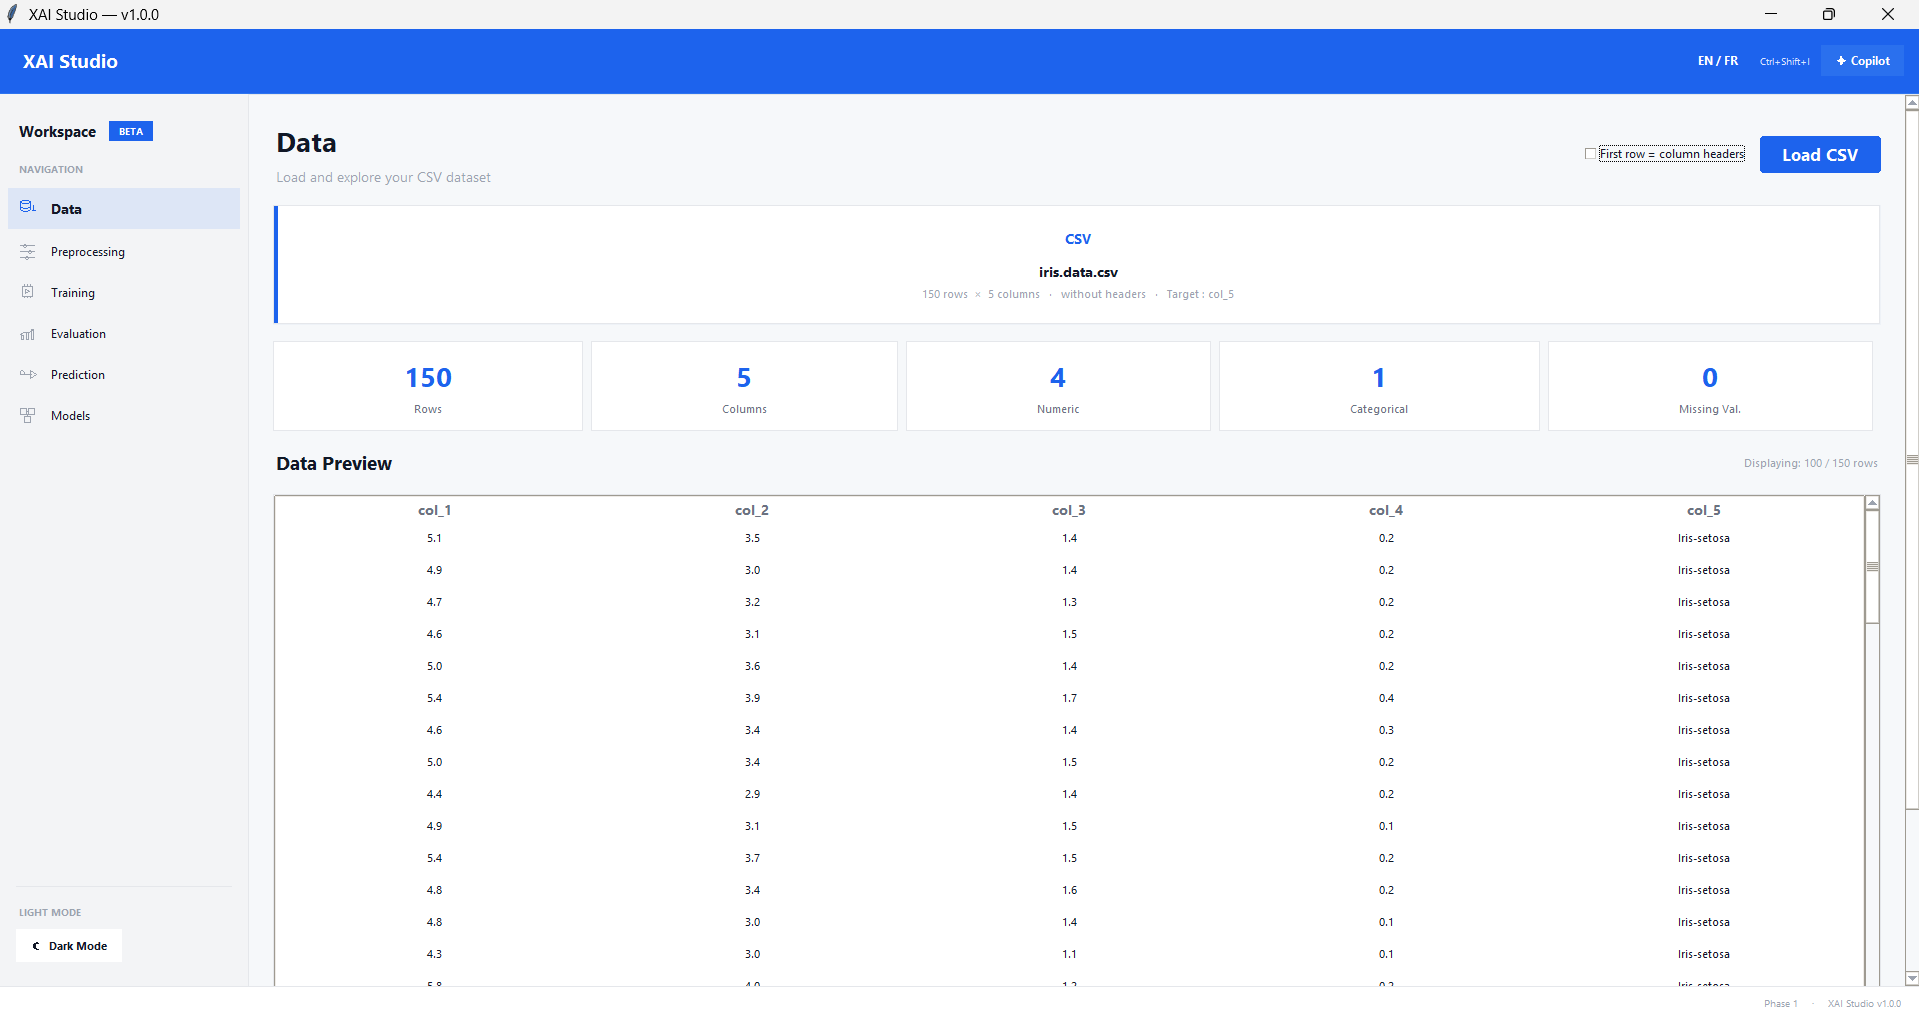
\includegraphics[width=\linewidth,keepaspectratio]{images/data.png}
    \caption{\'Ecran d'ingestion : aper\c{c}u tabulaire (\texttt{ttk.Treeview}), statistiques descriptives et s\'election de la cible.}
    \label{fig:data}
\end{figure}

L'utilisateur d\'ecouvre ici la \texttt{DataView}, une
\texttt{ttk.Frame} structur\'ee en deux colonnes par \texttt{grid()}:
\`a gauche un \texttt{ttk.Treeview} configur\'e en mode tabulaire
(colonnes dynamiques d\'eduites du \textit{DataFrame} pandas), \`a
droite un panneau \texttt{ttk.Frame} de m\'etadonn\'ees. Le
\textit{Treeview} est envelopp\'e dans un \texttt{tk.Canvas} +
\texttt{ttk.Scrollbar} bidirectionnels, technique classique de
Tkinter pour offrir un \textit{scroll} virtuel performant m\^eme sur
de tr\`es grands datasets. Les statistiques (taille, taux de valeurs
manquantes, type inf\'er\'e par colonne) sont rendues sous forme de
\og \textit{metric tiles} \fg{}\,---\,des \texttt{tk.Frame} arrondis
factoris\'es en composant r\'eutilisable. La s\'election de la cible
est mat\'erialis\'ee par une \texttt{ttk.Combobox} li\'ee \`a une
\texttt{StringVar} dont le \texttt{trace\_add('write')} d\'eclenche
imm\'ediatement la propagation \`a \texttt{PipelineService}.

% ─── Vue Preprocessing ───────────────────────────────────────────────
\subsection{Vue \og Pr\'eprocessing \fg{}\,---\,pipeline visuel}
\begin{figure}[H]
    \centering
    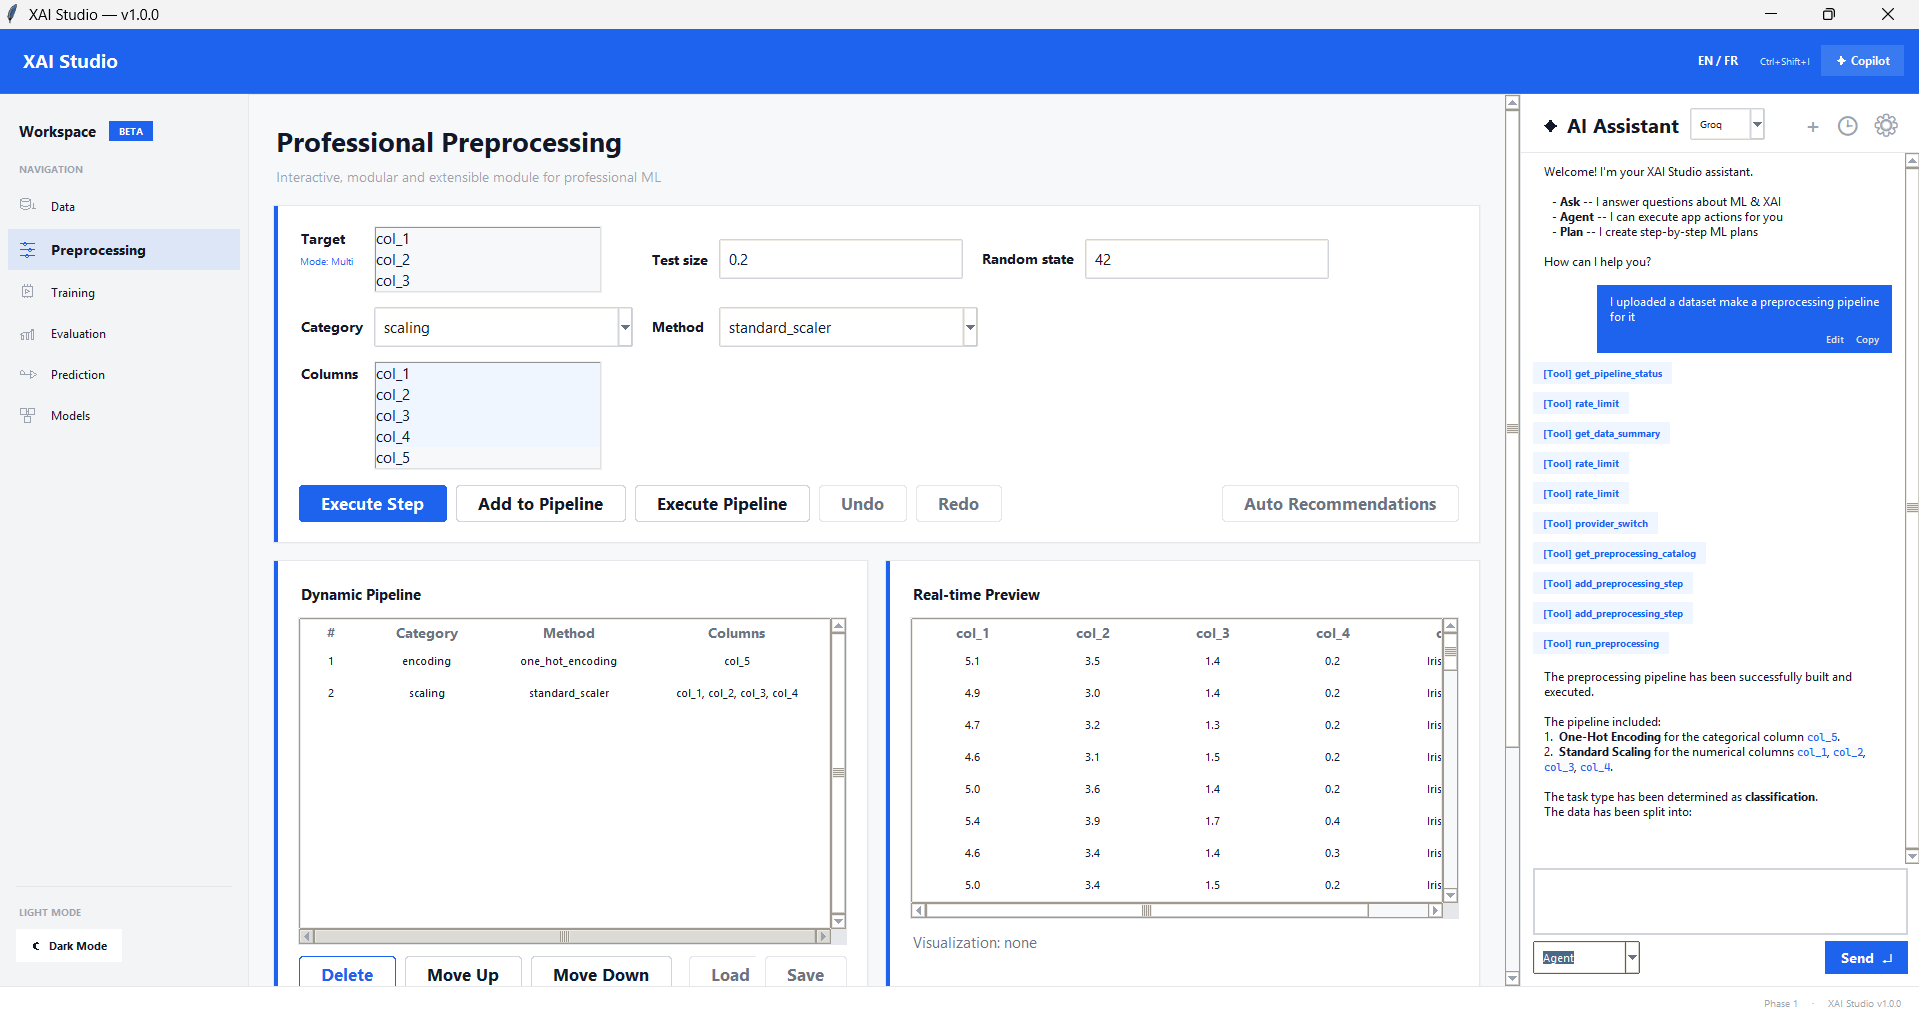
\includegraphics[width=\linewidth,keepaspectratio]{images/preprocessing.png}
    \caption{Studio de pr\'eprocessing : composition d'\'etapes (imputation, encodage, \textit{scaling}, \textit{split}) avec aper\c{c}u en temps r\'eel.}
    \label{fig:prep}
\end{figure}

La \texttt{PreprocessingView} est l'un des points o\`u Tkinter est
le plus sollicit\'e. Chaque \'etape du \textit{pipeline} est rendue
comme une \og carte \fg{} (un \texttt{tk.Frame} stylis\'e avec
bordure, \textit{padding} et \textit{badge} de statut) instanci\'ee
dynamiquement \`a la vol\'ee. La liste verticale est plac\'ee dans
un \texttt{tk.Canvas} dont la \textit{scrollregion} est recalcul\'ee
\`a chaque \texttt{<Configure>} pour s'adapter au nombre variable
d'\'etapes. Les contr\^oles par \'etape combinent
\texttt{ttk.Combobox}, \texttt{ttk.Spinbox} et
\texttt{ttk.Checkbutton}, tous reli\'es \`a des variables Tk pour un
binding r\'eactif. Une particularit\'e remarquable : cette m\^eme
vue est manipulable par l'agent IA via l'outil
\texttt{add\_preprocessing\_step}, ce qui implique qu'\textit{aucun
\'etat n'est pi\'eg\'e dans les \textit{widgets}}\,---\,la source de
v\'erit\'e reste le \texttt{PipelineService}, et l'UI se contente de
le refl\'eter.

% ─── Vue Training ────────────────────────────────────────────────────
\subsection{Vue \og Entra\^inement \fg{}\,---\,multi-mod\`eles asynchrone}
\begin{figure}[H]
    \centering
    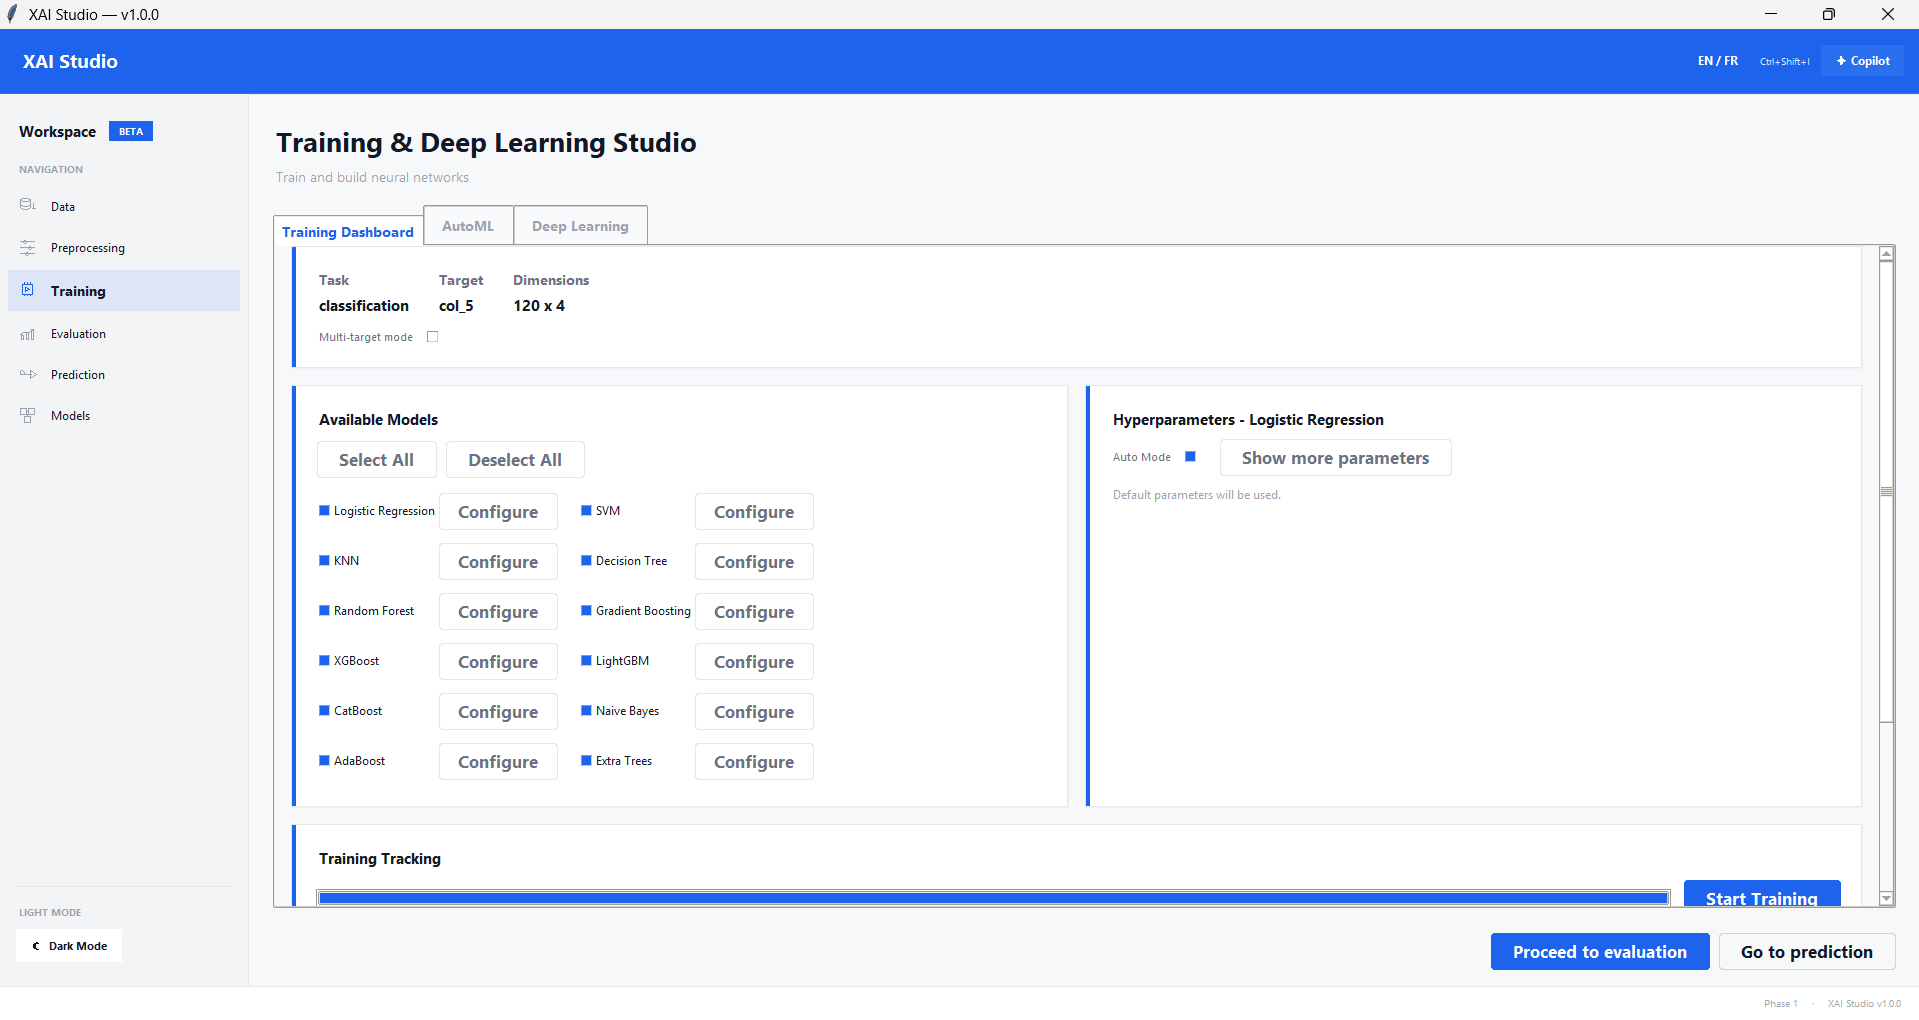
\includegraphics[width=\linewidth,keepaspectratio]{images/training.png}
    \caption{Studio d'entra\^inement : s\'election des mod\`eles, hyper-param\`etres et suivi de progression en direct.}
    \label{fig:train}
\end{figure}

La \texttt{TrainingView} illustre le pattern \og UI r\'eactive sur
calcul lourd \fg{}. L'utilisateur s\'electionne ses mod\`eles via une
matrice de \texttt{ttk.Checkbutton} reli\'ee \`a des
\texttt{BooleanVar}. Au lancement, l'entra\^inement est confi\'e \`a
un \texttt{threading.Thread} d\'emon ; chaque \textit{tick} de
progression est ensuite repouss\'e dans le \textit{mainloop} via
\texttt{root.after(0, callback)}, ce qui pr\'eserve la r\`egle d'or
de Tk (un seul \textit{thread} accroch\'e \`a la boucle d'\'ev\'enements).
Une \texttt{ttk.Progressbar} en mode \textit{determinate} affiche
l'avancement, doubl\'ee d'une \texttt{tk.Label} ETA. Les
hyper-param\`etres sont \'editables via des \texttt{ttk.Spinbox} et
\texttt{ttk.Entry} valid\'es \`a la sortie de focus
(\texttt{<FocusOut>}).

% ─── Vue Evaluation ──────────────────────────────────────────────────
\subsection{Vue \og \'Evaluation \fg{}\,---\,comparaison synth\'etique}
\begin{figure}[H]
    \centering
    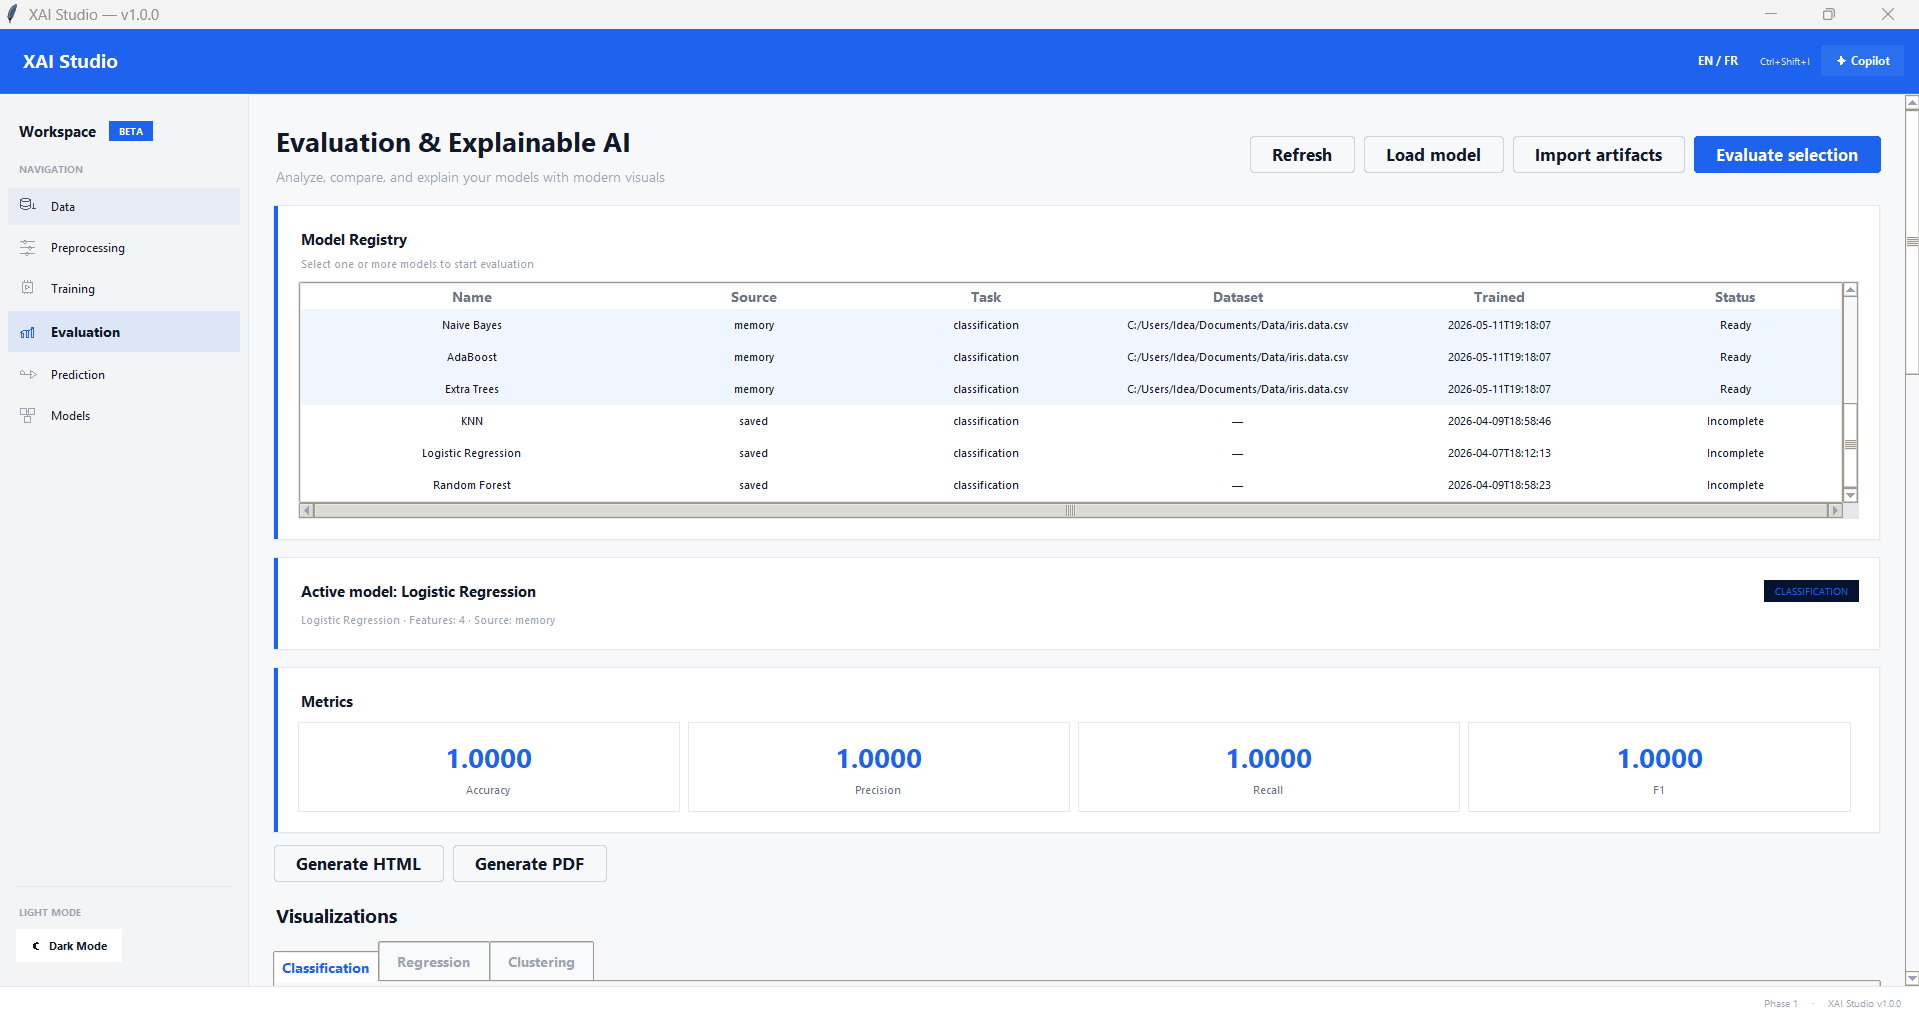
\includegraphics[width=\linewidth,keepaspectratio]{images/evaluation.png}
    \caption{Tableau comparatif des mod\`eles entra\^in\'es avec m\'etriques adapt\'ees \`a la t\^ache (classification/r\'egression).}
    \label{fig:eval}
\end{figure}

La vue d'\'evaluation pr\'esente un \texttt{ttk.Treeview} multi-colonnes
configur\'e par \texttt{column(\dots, anchor='center', stretch=True)}.
Les en-t\^etes sont triables : un \texttt{bind('<Button-1>',
sort\_handler)} sur chaque \textit{heading} d\'eclenche un tri stable
en place. Les m\'etriques (\textit{accuracy}, F1, RMSE, R\textsuperscript{2}\dots)
sont s\'electionn\'ees automatiquement selon le type de t\^ache
d\'etect\'e dans \texttt{PipelineService.evaluation\_kind}. Un
\textit{tag} de couleur souligne la ligne du meilleur mod\`ele,
appliqu\'e via \texttt{tree.tag\_configure('best', background=\dots)}.

% ─── Vue Models ──────────────────────────────────────────────────────
\subsection{Vue \og Mod\`eles \fg{}\,---\,catalogue persist\'e}
\begin{figure}[H]
    \centering
    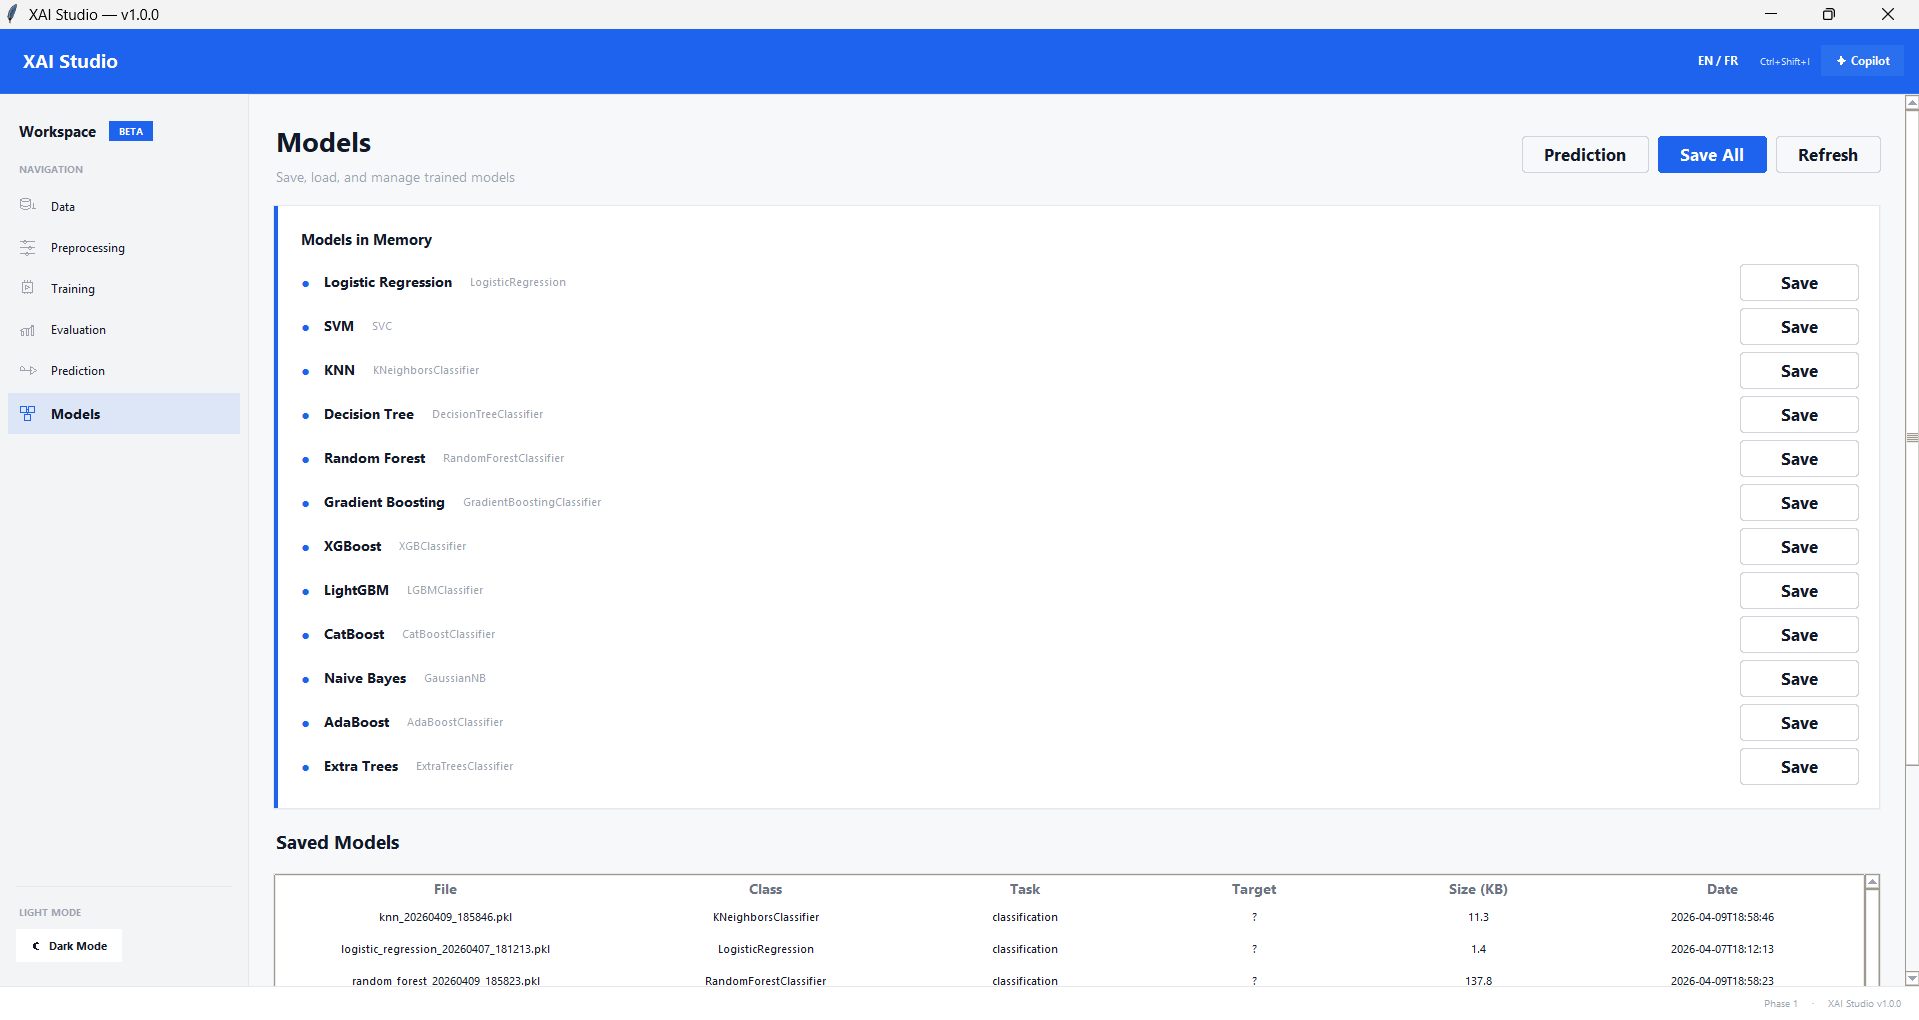
\includegraphics[width=\linewidth,keepaspectratio]{images/models.png}
    \caption{Catalogue des mod\`eles sauvegard\'es : m\'etadonn\'ees, sch\'ema d'entr\'ee et navigation rapide vers l'inf\'erence.}
    \label{fig:models}
\end{figure}

La \texttt{ModelsView} expose les artefacts \texttt{.pkl} pr\'esents
dans \texttt{models/saved/}. Chaque mod\`ele appara\^it sous forme
de \og fiche \fg{}\,---\,un \texttt{tk.Frame} arrondi
(\textit{rounded rectangle} dessin\'e via \texttt{tk.Canvas.create\_polygon}
avec les coins en \textit{smooth=True}) qui \'enum\`ere les m\'etadonn\'ees
charg\'ees \`a la vol\'ee : nom, algorithme, m\'etriques cl\'es, sch\'ema
d'entr\'ee. Les boutons d'action utilisent des \texttt{tk.Label}
\textit{clickable} (plut\^ot que \texttt{ttk.Button}) afin de
contr\^oler tr\`es finement la typographie et les \'etats hover via
\texttt{bind('<Enter>')} / \texttt{bind('<Leave>')}\,---\,un d\'etour
classique mais payant pour atteindre un rendu de niveau produit.

% ─── Vue Prediction ──────────────────────────────────────────────────
\subsection{Vue \og Pr\'ediction \fg{}\,---\,inf\'erence et what-if}
\begin{figure}[H]
    \centering
    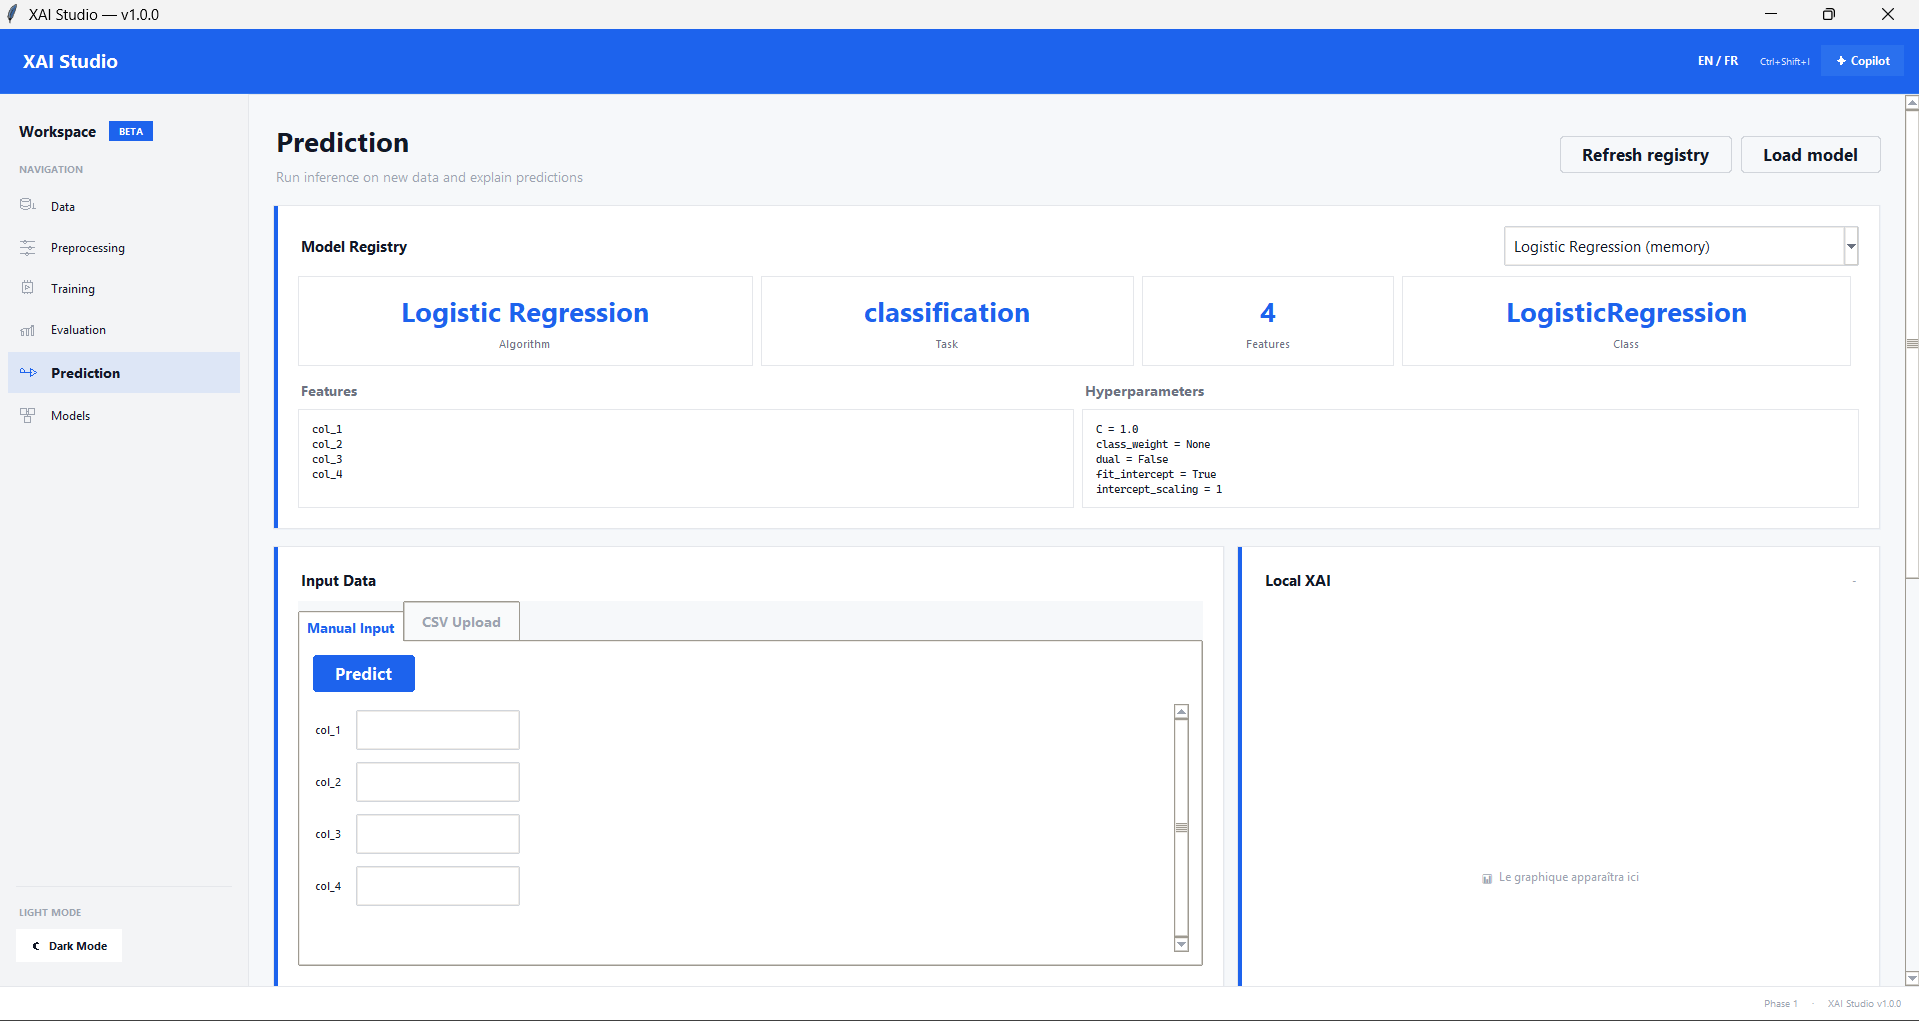
\includegraphics[width=\linewidth,keepaspectratio]{images/prediction.png}
    \caption{Module d'inf\'erence : saisie manuelle, import CSV par lot, analyse \textit{what-if} et explications SHAP locales.}
    \label{fig:pred}
\end{figure}

La \texttt{PredictionView} d\'emontre l'\'el\'egance qu'on peut
atteindre quand le sch\'ema d'entr\'ee est connu \`a l'avance.
Pour chaque \textit{feature} du mod\`ele charg\'e, la vue
g\'en\`ere automatiquement le \textit{widget} appropri\'e\,---\,
\texttt{ttk.Combobox} pour une variable cat\'egorielle (les choix
sont issus du \texttt{feature\_schema} persist\'e dans le
\texttt{.pkl}), \texttt{ttk.Spinbox} ou \texttt{tk.Scale} pour une
variable num\'erique continue. L'analyse \textit{what-if} utilise
des \texttt{tk.Scale} dont le \texttt{command=} d\'eclenche un
recalcul instantan\'e de la pr\'ediction et un re-rendu du graphique
SHAP via \texttt{matplotlib.FigureCanvasTkAgg} embarqu\'e dans la
hi\'erarchie Tk. Le \textit{batch} CSV passe par
\texttt{tkinter.filedialog.askopenfilename}, valid\'e c\^ot\'e
\texttt{services/}.

% ─────────────────────────────────────────────────────────────────────
% CHAPITRE 2 — ARCHITECTURE & INGENIERIE BACKEND
% ─────────────────────────────────────────────────────────────────────
\chapter{Architecture et ing\'enierie backend}

\section{Vue d'ensemble en trois couches}

L'architecture suit un mod\`ele en couches concentriques o\`u
chaque anneau ne d\'epend que de l'anneau imm\'ediatement
int\'erieur. Cette discipline\,---\,h\'erit\'ee de la \textit{Clean
Architecture}\,---\,explique la r\'esilience du projet aux
\'evolutions successives.

% ─── PLACEHOLDER : diagramme d'architecture en couches ───────────────
% Prompt fourni en fin de chat pour generation ulterieure
\begin{figure}[H]
    \centering
    \begin{tcolorbox}[
        colback=light, colframe=rule, boxrule=0.6pt,
        width=0.85\linewidth, arc=4pt,
        left=20pt, right=20pt, top=24pt, bottom=24pt
    ]
    \centering
    {\sffamily\color{muted}\itshape
    [Emplacement r\'eserv\'e\,---\,diagramme conceptuel\\
    de l'architecture en trois couches (\texttt{ui / services / core})\\
    \`a g\'en\'erer ult\'erieurement via DALL-E 3 / Midjourney.]}
    \end{tcolorbox}
    \caption{Vue conceptuelle de l'architecture en couches (\textit{placeholder}).}
    \label{fig:layered-arch}
\end{figure}

\begin{center}
\rowcolors{2}{light}{white}
\begin{tabular}{!{\color{accent}\vrule width 2pt}L{2.6cm} L{5cm} L{6.5cm}}
\arrayrulecolor{rule}\toprule
\textbf{Couche} & \textbf{Responsabilit\'e} & \textbf{D\'ependances autoris\'ees} \\
\midrule
\texttt{ui/}        & Tkinter / ttk, vues, composants, th\`emes \textit{light}/\textit{dark}, i18n FR/EN. & $\rightarrow$ \texttt{services/}                  \\
\texttt{services/}  & Orchestration m\'etier, agent IA, \textit{pipeline service}, clients LLM, i18n service.    & $\rightarrow$ \texttt{core/}                      \\
\texttt{core/}      & Logique ML pure : \textit{loader}, pr\'eprocessing, entra\^inement, \'evaluation, XAI, \textit{fairness}. & $\rightarrow$ \texttt{config/}, \texttt{utils/} \\
\bottomrule
\end{tabular}
\end{center}

\begin{techbox}{B\'en\'efice direct de cette discipline}
Aucun code Tkinter ne fuit vers \texttt{core/}. R\'eciproquement,
aucune r\'ef\'erence \textit{scikit-learn} ne contamine la couche
UI. Les services agissent comme \textit{façade} d'orchestration et
sont donc le \textbf{seul} point d'entr\'ee de l'agent IA, qui ne
peut pas \og tricher \fg{} en s'adressant directement aux mod\`eles.
\end{techbox}

\section{Agent (Copilot) : raisonnement et flux de d\'ecision}

\subsection{Architecture conceptuelle}

L'agent IA est mat\'erialis\'e par le module
\texttt{services/agent\_service.py}. Il fonctionne en boucle
agentique born\'ee (\texttt{MAX\_TOOL\_ITERATIONS = 8}) afin
d'\'eviter tout cycle infini.

\begin{figure}[H]
    \centering
    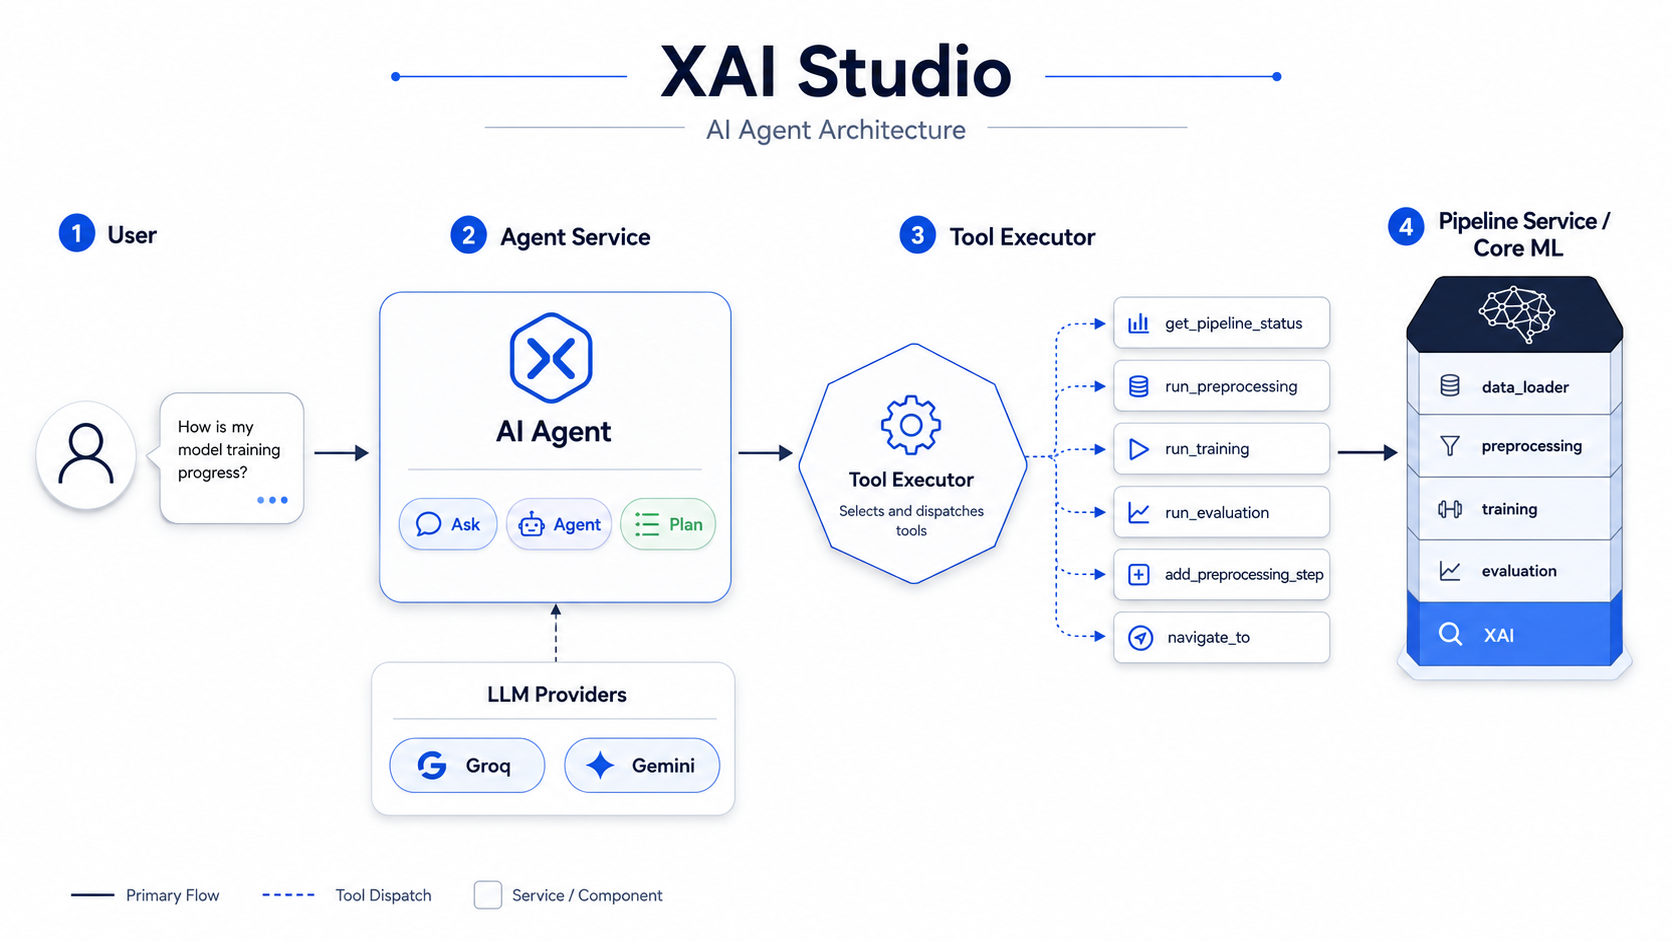
\includegraphics[width=0.95\linewidth,keepaspectratio]{images/agent_architecture_diagram.png}
    \caption{Architecture conceptuelle de l'agent\,---\,position du \textit{Copilot} entre l'UI Tkinter, le \textit{ToolExecutor}, le \textit{PipelineService} et les \textit{providers} LLM externes.}
    \label{fig:agent-arch}
\end{figure}

Le sch\'ema ci-dessus met en \'evidence quatre constats
d'ing\'enierie majeurs :

\begin{enumerate}
    \item \textbf{L'agent n'est jamais un raccourci}\,---\,m\^eme en
        mode \og Agent \fg{}, il invoque \texttt{PipelineService}
        comme l'aurait fait un utilisateur cliquant dans l'UI.
    \item \textbf{Le \texttt{ToolExecutor} est l'unique point de
        dispatch}\,---\,il valide les arguments, capture les
        exceptions et standardise les r\'eponses. C'est \'egalement
        l\`a que l'on inject\^et un \textit{rate-limiter} ou un
        journal d'audit si besoin.
    \item \textbf{Les \textit{providers} (Groq, Gemini) sont
        interchangeables}\,---\,le contrat est r\'eduit \`a une
        m\'ethode \texttt{chat(messages, tools)} qui retourne une
        structure unifi\'ee.
    \item \textbf{L'UI ne sait rien des LLM}\,---\,le
        \texttt{AgentPanel} (un \texttt{tk.Frame} avec une zone de
        chat \texttt{tk.Text} \`a \textit{tags} de couleurs et un
        \texttt{ttk.Entry} de saisie) ne communique qu'avec
        \texttt{AgentService}, jamais directement avec les API.
\end{enumerate}

\subsection{Trois modes d'op\'eration}
\begin{description}[font=\sffamily\bfseries\color{accent}]
    \item[Ask]
        R\'eponses purement conversationnelles, sans appel d'outil.
        Le \textit{system prompt} interdit explicitement le \textit{tool-calling}.
        Cas d'usage : aide p\'edagogique, FAQ XAI.

    \item[Agent]
        Mode autonome avec \textit{tool-calling} activ\'e. L'agent
        peut lire l'\'etat du \textit{pipeline}, ex\'ecuter des
        actions et naviguer entre vues. La directive critique
        \og \textit{Visual Pipeline Construction} \fg{} le pousse
        \`a privil\'egier la construction visuelle du
        \textit{pipeline} plut\^ot qu'un appel monolithique.

    \item[Plan]
        Mode r\'eflexion : l'agent produit un plan structur\'e
        \textit{avant} ex\'ecution. Adapt\'e aux \textit{workflows}
        complexes o\`u l'utilisateur veut valider la d\'emarche
        avant de l'appliquer.
\end{description}

\section{Tools et flux d'ex\'ecution}

\subsection{Orchestration technique}

Le contrat de \textit{tool-calling} suit le sch\'ema OpenAI standard,
ce qui garantit la portabilit\'e vers tout \textit{provider}
compatible. Le \texttt{ToolExecutor} d\'esigne la couche qui
transforme l'intention de l'agent en action concr\`ete.

\begin{figure}[H]
    \centering
    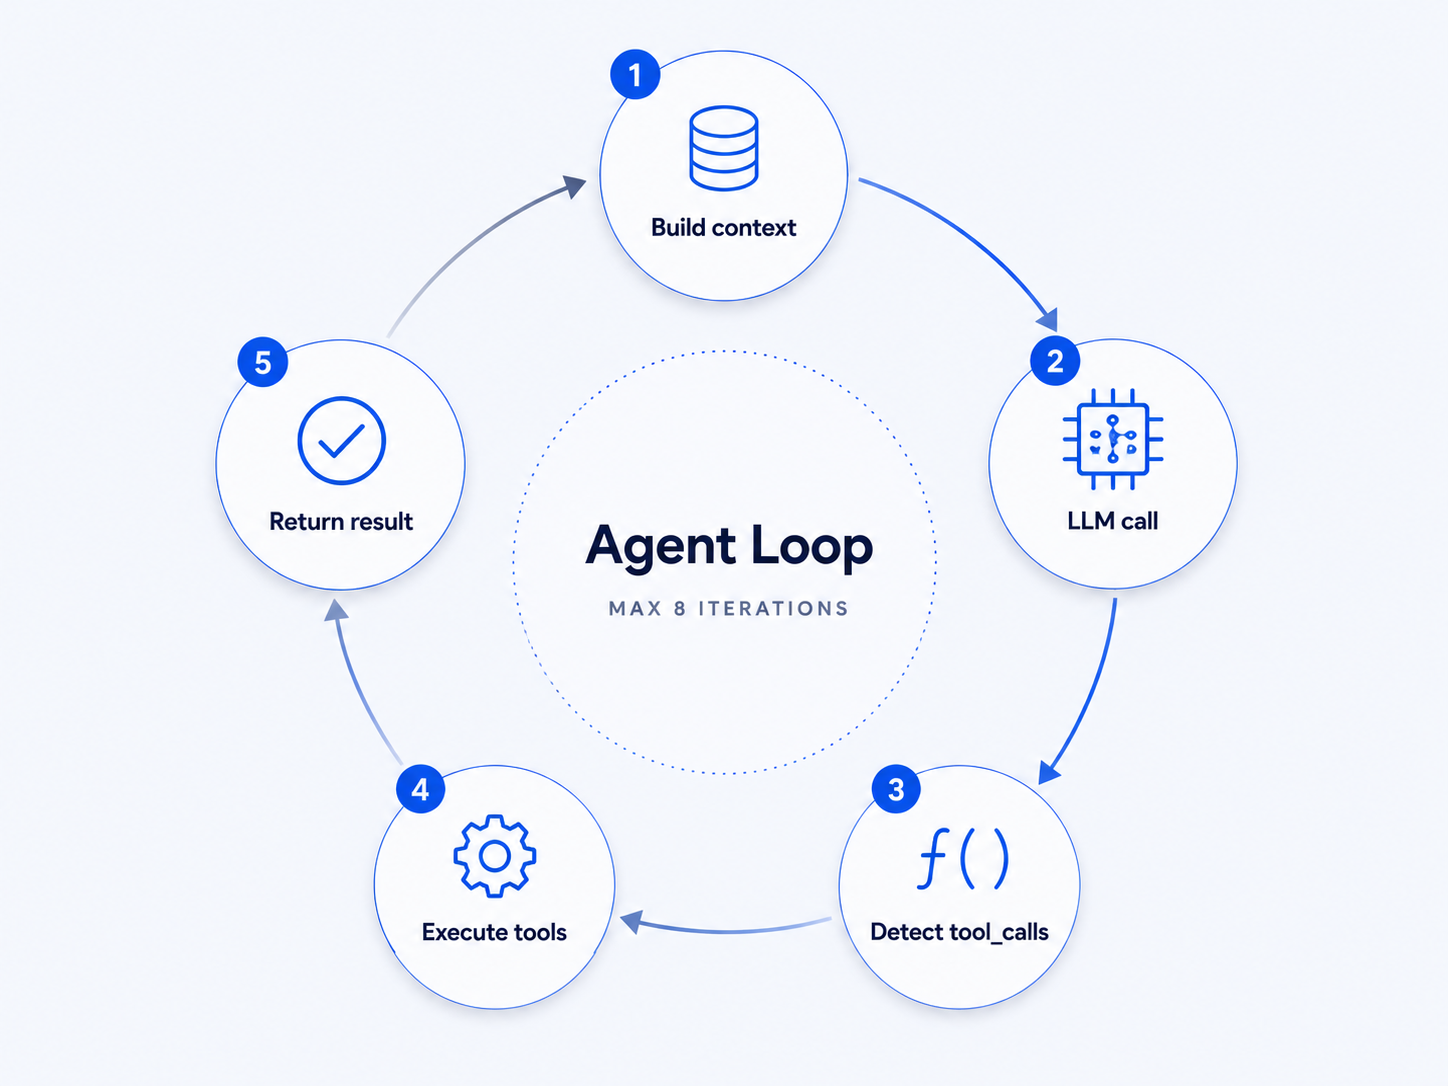
\includegraphics[width=0.95\linewidth,keepaspectratio]{images/tool_calling_flow.png}
    \caption{Flux de \textit{tool-calling}\,---\,boucle agentique compl\`ete, de la r\'eception du message utilisateur \`a la r\'eponse finale, en passant par la d\'etection des \texttt{tool\_calls} et leur ex\'ecution.}
    \label{fig:tool-flow}
\end{figure}

\textbf{Lecture du sch\'ema.} La boucle proc\`ede en cinq \'etapes
strictement ordonn\'ees~:

\begin{enumerate}
    \item \textbf{Build context}\,---\,\texttt{AgentService} compile
        l'\'etat courant (statut du \textit{pipeline}, langue de
        l'utilisateur, mode actif) puis le pr\'efixe au message.
    \item \textbf{LLM call}\,---\,le \textit{provider} re\c{c}oit les
        messages plus le catalogue d'outils.
    \item \textbf{Detect tool\_calls}\,---\,si la r\'eponse contient
        des appels, ils sont parse\'es ; sinon, le \textit{flow}
        court-circuite vers l'\'etape 5.
    \item \textbf{Execute tools}\,---\,le \texttt{ToolExecutor}
        invoque les m\'ethodes correspondantes de
        \texttt{PipelineService}, capture les erreurs et r\'einjecte
        les r\'esultats sous forme de messages \texttt{tool} dans
        l'historique.
    \item \textbf{Return result}\,---\,une fois la boucle satisfaite
        (ou la limite de 8 it\'erations atteinte), la r\'eponse
        finale est envoy\'ee \`a l'UI, qui la rend dans son
        \texttt{tk.Text} avec mise en forme markdown maison.
\end{enumerate}

\subsection{Catalogue d'outils}

Le registre \texttt{services/agent\_tools.py} d\'eclare quatorze
outils, chacun \textit{wrapper} fin autour d'une m\'ethode
\texttt{PipelineService} existante. Cette discipline garantit qu'il
n'existe aucune logique ML expos\'ee uniquement \`a l'agent.

\begin{center}
\rowcolors{2}{light}{white}
\begin{tabular}{!{\color{accent}\vrule width 2pt}L{6cm} L{8cm}}
\arrayrulecolor{rule}\toprule
\textbf{Outil} & \textbf{R\^ole} \\
\midrule
\texttt{get\_pipeline\_status}           & \'Etat global (donn\'ees, cible, pr\'eprocessing, mod\`eles, \'evaluation). \\
\texttt{get\_data\_summary}              & Forme, types, valeurs manquantes, statistiques descriptives. \\
\texttt{get\_columns}                    & Liste exhaustive des colonnes du dataset. \\
\texttt{set\_target\_columns}            & D\'efinition de la (des) cible(s) supervis\'ee(s). \\
\texttt{get\_preprocessing\_recommendations} & Suggestions fond\'ees sur l'analyse du dataset. \\
\texttt{get\_preprocessing\_issues}      & D\'etection des probl\`emes bloquants pr\'e-entra\^inement. \\
\texttt{get\_preprocessing\_catalog}     & Liste exhaustive des \'etapes de pr\'eprocessing disponibles. \\
\texttt{add\_preprocessing\_step}        & Ajout dynamique d'une \'etape au \textit{pipeline} visuel. \\
\texttt{run\_preprocessing}              & D\'eclenchement de l'ex\'ecution du \textit{pipeline}. \\
\texttt{get\_available\_models}          & Liste des mod\`eles candidats selon la t\^ache d\'etect\'ee. \\
\texttt{run\_training}                   & Entra\^inement multi-mod\`eles asynchrone. \\
\texttt{run\_evaluation}                 & Calcul des m\'etriques sur le jeu de test. \\
\texttt{get\_comparison\_table}          & R\'ecup\'eration du tableau comparatif des performances. \\
\texttt{navigate\_to}                    & Navigation programm\'ee vers une vue Tkinter. \\
\bottomrule
\end{tabular}
\end{center}

\begin{techbox}{Pourquoi le \textit{wrapper} plut\^ot que l'acc\`es direct ?}
Chaque outil est une coquille fine. Avantages~: (i) le m\^eme code
m\'etier est ex\'ecut\'e qu'on vienne de l'agent ou de l'UI ; (ii)
les invariants sont test\'es une seule fois c\^ot\'e
\texttt{PipelineService} ; (iii) un ajout futur (audit, t\'el\'em\'etrie,
\textit{rate-limit}) se branche en un seul endroit.
\end{techbox}

\section{M\'emoire : contexte et persistance}

La m\'emoire conversationnelle se d\'ecline sur trois plans, chacun
con\c{c}u pour r\'esister \`a des d\'efaillances diff\'erentes~:

\begin{description}[font=\sffamily\bfseries\color{accent}]
    \item[M\'emoire de session (volatile)]
        L'historique structur\'e (\texttt{user},
        \texttt{assistant}, \texttt{tool}) vit en m\'emoire vive au
        sein de \texttt{AgentService}. Il est servi tel quel au
        \textit{provider} lors de chaque tour, sans tronquage tant
        que la fen\^etre de contexte le permet.

    \item[Persistance disque (JSON)]
        Chaque conversation est s\'erialis\'ee dans
        \texttt{data/chats/} sous forme JSON. Cela autorise la
        reprise de session apr\`es un red\'emarrage et constitue la
        base d'un futur historique consultable.

    \item[Reprise inline d'un prompt]
        Un bouton \og Edit \fg{} sur chaque message utilisateur le
        recharge dans la \texttt{ttk.Entry} d'envoi (via un
        \texttt{bind('<Button-1>', \dots)} sur la \textit{tag}
        correspondante du \texttt{tk.Text}). Petite touche UX qui
        \'evite la recopie manuelle.
\end{description}

\section{Providers IA : Groq et Gemini}

\subsection{Un client unifi\'e sans d\'ependance externe}

Le module \texttt{services/llm\_client.py} expose une interface
unique pour les deux \textit{providers}. Le choix radical~:
n'utiliser que \texttt{urllib} de la biblioth\`eque standard. Cela
\'elimine toute d\'ependance \texttt{pip} pour la couche LLM,
all\`ege les installations et neutralise les risques de
\textit{breaking changes} c\^ot\'e SDK tiers.

\vspace{0.8em}
\begin{center}
\begin{tabular}{ccc}
\begin{minipage}{0.30\linewidth}
    \centering
    
\includegraphics[width=\linewidth,keepaspectratio]{images/grok_logo.png}
\end{minipage}
&
\hspace{0.6cm}
&
\begin{minipage}{0.30\linewidth}
    \centering
    
\includegraphics[width=\linewidth,keepaspectratio]{images/gemini_logo.png}
\end{minipage}
\\[8pt]
{\sffamily\bfseries\color{accent}\large Groq}
&
&
{\sffamily\bfseries\color{accent}\large Google Gemini}
\\
{\sffamily\small\color{muted}llama-3.3-70b-versatile}
&
&
{\sffamily\small\color{muted}gemini-pro / gemini-1.5}
\end{tabular}
\end{center}
\vspace{0.8em}

\subsection{Int\'egration Groq\,---\,r\'esolution d'un blocage Cloudflare}

\texttt{GroqProvider} cible l'endpoint OpenAI-compatible
\texttt{https://api.groq.com/openai/v1/chat/completions}. Durant
l'int\'egration, le service renvoyait syst\'ematiquement un
\textit{403 Forbidden} d\^u \`a un filtre Cloudflare anti-bot.
Le diagnostic a r\'ev\'el\'e que l'absence d'en-t\^ete
\texttt{User-Agent} suffisait \`a d\'eclencher le blocage. La
correction\,---\,ajout d'un \texttt{User-Agent: XAI-Studio/1.0}
explicite\,---\,a r\'esolu le probl\`eme et constitue d\'esormais le
comportement par d\'efaut. Une distinction est par ailleurs faite
entre \texttt{RateLimitError} et \texttt{LLMError} g\'en\'erique
pour permettre un \textit{back-off} adapt\'e dans
\texttt{AgentService}.

\subsection{Int\'egration Gemini\,---\,r\'eparation du function-calling}

\texttt{GeminiProvider} consomme l'API Google \textit{Generative AI}.
La d\'erive technique observ\'ee \'etait subtile~: Gemini renvoyait
des erreurs HTTP 400 pendant l'ex\'ecution du \textit{tool-calling}.
Le format attendu c\^ot\'e Google \'etait un \textit{Protobuf Struct}
natif, l\`a o\`u nous transmettions une cha\^ine JSON
\og\,stringifi\'ee\,\fg{}. La couche d'adaptation a donc \'et\'e modifi\'ee
pour appeler \texttt{json.loads} systematiquement sur les arguments
avant transmission, restaurant ainsi la conformit\'e.

\subsection{Configuration locale et s\'ecurit\'e}

Les cl\'es API et le \textit{provider} actif sont persist\'es dans
\texttt{config/agent.json}. Ce fichier est explicitement ignor\'e
par \texttt{.gitignore} : aucune cl\'e n'a fui dans l'historique
git. C\^ot\'e UI, une \texttt{tk.Toplevel} d\'edi\'ee
(\texttt{AgentSettingsDialog}) permet de basculer entre
\textit{providers}, de valider la cl\'e en ligne (appel HTTP de
\textit{ping}) et de r\'ecup\'erer dynamiquement la liste des
mod\`eles disponibles.

% ─────────────────────────────────────────────────────────────────────
% CHAPITRE 3 — EVOLUTION DU PROJET
% ─────────────────────────────────────────────────────────────────────
\chapter{\'Evolution du projet et discipline d'ing\'enierie}

L'analyse de l'historique \texttt{git} permet de relire le projet
sous l'angle de la \textit{discipline d'ing\'enierie} : chaque jalon
correspond \`a une livraison fonctionnelle qui respecte les
contrats d'architecture pos\'es au d\'epart. Cette section synth\'etise
l'\'evolution en cinq grandes phases.

\section{Phase 1\,---\,Fondations architecturales}

\begin{milestonebox}{Mise en place de la structure modulaire}
\textbf{c9c73cb} -- \textit{22 fichiers r\'epartis sur 6 couches architecturales}.
D\`es le premier \textit{commit}, le projet adopte une organisation
en couches s\'epar\'ees. Cette d\'ecision fondatrice explique la
totalit\'e des choix ult\'erieurs~: aucune r\'egression d'architecture
n'a \'et\'e observ\'ee par la suite.
\end{milestonebox}

\begin{milestonebox}{Pull request inter-branches}
\textbf{0084e52 / 90377a3} -- \textit{ph2-firstpush} merg\'e depuis
la branche \texttt{Fatima-Ezzahrae\_\_AKEBLI}. La mise en place
imm\'ediate d'un \textit{workflow} de \textit{feature branches} +
\textit{pull request} t\'emoigne d'une rigueur de gestion de version
inhabituelle \`a ce stade d'un projet \'etudiant.
\end{milestonebox}

\section{Phase 2\,---\,Maturation UI et premier \'elan ML}

\begin{milestonebox}{Pr\'eprocessing et rendu HiDPI}
\textbf{a46ee0b} -- \textit{Improve preprocessing UI and DPI rendering}.
Introduction de la d\'etection automatique de DPI et du
\textit{scaling} Tk. Sans cette correction pr\'ecoce, les \'ecrans
4K rendaient une UI floue.
\end{milestonebox}

\begin{milestonebox}{Training Studio, AutoML et NN Builder}
\textbf{3cb7fb3} -- \textit{Add training progress ETA, basic AutoML, and NN Builder MVP}.
Le \texttt{TrainingView} h\'erite du suivi temps r\'eel, et un
\textit{prototype} d'AutoML appara\^it. Le \textit{NN Builder}
amorce une approche \og programmation visuelle \fg{} qui pr\'efigure
le \textit{pipeline} visuel manipulable par l'agent.
\end{milestonebox}

\begin{milestonebox}{Harmonisation de la navigation}
\textbf{a157e91} -- \textit{Update UI flow navigation and preprocessing layout}.
Refonte du \texttt{Sidebar} et r\'eorganisation des
\texttt{ttk.Frame} pour homog\'en\'eiser la navigation\,---\,une
\'etape critique pour la coh\'erence ergonomique.
\end{milestonebox}

\begin{milestonebox}{Revamp du Training Studio}
\textbf{d337aec} -- \textit{Revamp training studio UI and NN builder}.
Seconde it\'eration majeure du studio d'entra\^inement~: gestion
plus fine des hyper-param\`etres, am\'elioration de la composition
visuelle.
\end{milestonebox}

\begin{milestonebox}{Modules d'\'evaluation et XAI}
\textbf{df5a492} -- \textit{Add evaluation and XAI dashboard modules}.
Apparition du tableau de bord XAI (SHAP, LIME, PDP) qui constitue
la \textit{signature} du projet et fonde son identit\'e
\textit{Explainable AI}.
\end{milestonebox}

\begin{milestonebox}{Simplification du Training et navigation Eval}
\textbf{a8df019} -- \textit{Simplify training view and add evaluation nav}.
Mouvement de simplification courageux~: le \textit{Training Studio}
se concentre sur l'essentiel et c\`ede les fonctions secondaires
\`a l'\'evaluation.
\end{milestonebox}

\section{Phase 3\,---\,Industrialisation du module de pr\'ediction}

\begin{milestonebox}{Pr\'ediction \og schema-aware \fg{}}
\textbf{e0520ce} -- \textit{Prediction module with categorical input support and schema-aware transformations}.
Jalon strat\'egique~: le nouveau module de pr\'ediction utilise les
m\'etadonn\'ees s\'erialis\'ees dans le mod\`ele (\texttt{input\_feature\_names},
\texttt{categorical\_columns}, \texttt{feature\_schema}) pour rendre
le bon \textit{widget} Tk \`a la vol\'ee (\texttt{ttk.Combobox} pour
les cat\'egories, \texttt{tk.Scale} pour les num\'eriques).
La transformation appliqu\'ee en inf\'erence est strictement la
m\^eme que celle de l'entra\^inement\,---\,\textbf{c'est la garantie
silencieuse} qui pr\'evient les bugs les plus fr\'equents en
production ML.
\end{milestonebox}

\section{Phase 4\,---\,L'agent IA comme couche d'orchestration}

\begin{milestonebox}{Int\'egration du Copilote}
\textbf{fb7a9d9} -- \textit{integrate persistent AI Copilot agent with dynamic tool-calling}.
Le \textit{commit body} se lit comme une feuille de route d'ing\'enierie~:
panneau persistant, client unifi\'e Groq + Gemini sans d\'ependance
externe, validation d'API en ligne, r\'esolution du \textit{403
Forbidden} Cloudflare, r\'eparation du \textit{function calling}
Gemini, outils de manipulation dynamique du \textit{pipeline}, bouton
\og Edit \fg{} sur les prompts, retrait strict des \textit{emojis}
pour un rendu professionnel, et stockage local \textit{git-ignored}
des cl\'es API. \textbf{Quatre bugs externes d\'ebusqu\'es et
corrig\'es} en un seul jalon\,---\,une masterclass de
\textit{integration engineering}.
\end{milestonebox}

\begin{milestonebox}{Internationalisation compl\`ete FR / EN}
\textbf{1681540} -- \textit{Full English / French localization across all UI views}.
D\'eploiement d'un \texttt{I18nService} centralis\'e. Toutes les
cha\^ines des vues sont d\'esormais r\'esolues dynamiquement, ce
qui suppose une discipline strict~: \textit{zero hard-coded string}.
La pr\'ef\'erence est persist\'ee dans \texttt{config/lang.json}.
\end{milestonebox}

\section{Phase 5\,---\,Consolidation finale}

\begin{milestonebox}{Pipeline dynamique pilot\'e par l'agent}
\textbf{2f987de} -- \textit{enable agent to add steps directly to dynamic pipeline}.
L'agent acquiert la capacit\'e d'ajouter directement des \'etapes
au \textit{pipeline} visuel. C'est la jonction finale entre
raisonnement LLM et UI Tkinter\,---\,et la d\'emonstration que
notre architecture supportait ce pas suppl\'ementaire sans
refactoring lourd.
\end{milestonebox}

\begin{milestonebox}{Robustification multi-cibles}
\textbf{f768882} -- \textit{stabilize multi-target training, evaluation, and dynamic splits}.
Hardening du \textit{pipeline}~: prise en charge de plusieurs
cibles, \textit{splits} dynamiques, fiabilisation de l'\'evaluation.
\end{milestonebox}

\begin{milestonebox}{Mise \`a jour documentaire finale}
\textbf{461e9f2} -- \textit{Updated README with latest modifications}.
Mise en coh\'erence du \texttt{README} avec l'\'etat livr\'e.
Petit \textit{commit}, mais signal cl\'e de la rigueur~: la
documentation suit le code.
\end{milestonebox}

\section{Synth\`ese et conclusion}

\begin{pitchbox}
\sffamily\color{primary}
XAI Studio prouve trois propositions \`a la fois~:

\textbf{1.} Tkinter, manipul\'e avec discipline (\texttt{ttk.Style}
dynamique, \textit{scaling} HiDPI, conteneurs scrollables sur
\texttt{Canvas}, \textit{threading} cadenc\'e par \texttt{after()})
peut livrer une exp\'erience desktop de qualit\'e
professionnelle\,---\,et ce, sans framework tiers.

\textbf{2.} Une architecture en couches strictement respect\'ee
n'est pas un luxe~: elle est ce qui a permis d'int\'egrer
successivement le module XAI, le module de pr\'ediction
\textit{schema-aware}, l'agent LLM et l'i18n compl\`ete \textbf{sans
jamais r\'e\'ecrire la couche pr\'ec\'edente}.

\textbf{3.} Un agent LLM, lorsqu'il est conçu comme \textit{client
d'une API m\'etier} plut\^ot que comme \textit{tunnel direct vers
le code}, ne d\'estabilise pas l'architecture\,---\,il l'enrichit.
\end{pitchbox}

L'historique git, lu dans son ensemble, raconte une histoire de
prise de d\'ecisions techniques justes au bon moment~: une
fondation modulaire d\`es le premier \textit{commit}, des
am\'eliorations incr\'ementales successivement valid\'ees par des
\textit{pull requests}, et une derni\`ere phase de stabilisation qui
ferme le projet sur un livrable robuste, document\'e et internationalis\'e.
La synergie entre l'\'el\'egance d'une UI Tkinter pouss\'ee dans ses
retranchements et la rigueur d'un \textit{backend} orient\'e
services positionne XAI Studio comme un cas d'\'etude
particuli\`erement convaincant des bonnes pratiques d'ing\'enierie
logicielle appliqu\'ees \`a un produit de \textit{data science}
professionnel.

\end{document}
